% !TEX root = ../main.tex
\documentclass[../main.tex]{subfiles}

\begin{document}
\section{Secure Command Line Interface}

The command line interface of the application depends on communication via a Unix domain socket \cite{unix_domain_socket},
guaranteeing secure communication accessible only by having system access to the running application.
The location of the socket alogiside the feature toogle is defined by the application configuration file.

\subsection{Application config system}

The application configuration files are stored in YAML file format \cite{yaml}.
Configuration system is hierarchical, if files are stored in multiple locations they are merged together.
The config files can have either \textbf{.yml} or \textbf{.yaml} file extension.
Name of the file can be one of the following:
\begin{itemize}
  \item \textbf{hydra}
  \item \textbf{hydra-config}
  \item \textbf{hydra.config}
\end{itemize}

Additionally, each configuration file can have a \textbf{.local} added before the file extension, e.g. \textbf{hydra.local.yml}. This is reffered to as \textbf{local} configuration file.
Also, a dot can be added to the start of the file name, e.g. \textbf{.hydra.yml}. This is reffered to as \textbf{hidden} configuration file. Other configuration files are reffered to as \textbf{normal} or \textbf{standard} configuration files.

When configuration files are merged they are merged in the following order:
\begin{enumerate}
  \item \textbf{local} configuration files
  \item \textbf{hidden} configuration files
  \item \textbf{normal} configuration files
\end{enumerate}

Local configuration files override entries in hidden configuration files, which override entries in normal configuration files.

The configuration files can be stored in the following locations:
\begin{itemize}
  \item \textbf{\$HOME} directory
  \item \textbf{\$HOME/.config/hydra} directory
  \item \textbf{\$PWD} (current working directory) of server process
  \item \textbf{config} directory of the monorepository
\end{itemize}

The code that handles merging and handling of the configuration files is located in the \textbf{common} package under \textbf{src/server/coonfig} directory.

\begin{figure}[H]
  \centering
  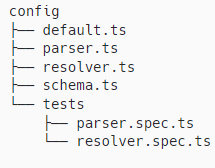
\includegraphics{file-tree/config-tree.png}
  \caption{File tree of files that implement the configuration system}
\end{figure}

The \texttt{defailt.ts} file contains the default configuration values that are used if no configuration file is found.

\begin{listing}[H]
  \tsfile{implementation/code/cli/config-default.ts}
  \caption{Contents of \texttt{default.ts} file}
\end{listing}

The \texttt{resolver.ts} file contains the logic that searches for configuration files and determinate the order in which they are to be loaded and merged.
To load a configuratation file \texttt{fromFile} static method from \texttt{HydraConfig} class is used. It takes a path to the configuration file and returns a \texttt{HydraConfig} instance.

\begin{listing}[H]
  \tsfile{implementation/code/cli/config-parser.ts}
  \caption{\texttt{parser.ts} file containing the \texttt{HydraConfig} class}
\end{listing}

The config file structure is validated using schema defined in \texttt{schema.ts} file.
To define and validate the schema \texttt{zod} library is used \cite{zod}.

\begin{listing}[H]
  \tsfile{implementation/code/cli/config-schema.ts}
  \caption{Config schema definition using \texttt{zod} library}
\end{listing}

The \texttt{HydraConfig} class is employed by both the \textbf{backend} and \textbf{cli} application to load configuration files.
If the \textbf{enable} flag under \textbf{socket} entry is set \textbf{true} then the unix socket is created and the \textbf{path} value is used as the path to the socket.
In contrast, when the \textbf{enable} flag is configured as \textbf{false}, the socket is not generated.
This absence of a socket results in a communication breakdown between the \textbf{cli} application and the \textbf{backend} application, effectively disabling this feature.

\begin{listing}[H]
  \yamlfile{implementation/code/cli/config-example.yml}
  \caption{Example hydra configuration file with enabled socket communication}
\end{listing}

\subsection{Socket creation and API definition}

The management api over unix socket is created upon application satrtup if feature is enabled in the configuration file.

\begin{listing}[H]
  \tsfile{implementation/code/cli/backend-init.ts}
  \caption{Backend initialization code}
\end{listing}

The management module exposes a signel controller which define two routes:

\begin{itemize}
  \item \textbf{accounts/create-admin-account} - creates account with admin privileges
  \item \textbf{accounts/create-standard-account} - creates standard account subjected to permission system
\end{itemize}

This controler does not use any authentication or authorization middleware, as it is not exposed to the internet and is only accessible by the \textbf{cli} application.

\subsection{CLI application}

The command line application was created using the \texttt{nestjs-commander} library \cite{nestjs-commander}, which allow creating CLI application using
existijng nestjs constructs like services and dependency injection.

Each command is represented by a class that extends the \texttt{CommandRunner} class from the \texttt{nestjs-commander} library.
These classes have to at least implement the \texttt{run} method which is invoked when the command is executed.
Additionaly command can define its name, description, arguments and options.

Arguments and options represent the user input that is passed to the command.
Arguments are positional and are passed to the command in the order they are defined.
Options are passed to the command using the \texttt{--option-name} syntax.
It is possible to define a short option name using the \texttt{-o} syntax.

\begin{listing}[H]
  \tsfile{implementation/code/cli/command-example.ts}
  \caption{Fragemnt of class defining command that creates new admin user}
\end{listing}

Additionaly additional questions can be asked to user to fill in the missing arguments or options that were not passed to the command.
This is implemented thorugh class that is decorated with \texttt{QuestionSet} decorator. Each method of this class represents a question that is asked to the user to fill in the missing data.

\begin{listing}[H]
  \tsfile{implementation/code/cli/question-example.ts}
  \caption{Fragemnt of class defining question set that asks user for missing data}
\end{listing}

To invoke \texttt{cli} application, the \texttt{Node.js} interpreter is invoked on the compiled entrypoint file.

\begin{listing}[H]
  \begin{bashcode}
    node dist/main.js
  \end{bashcode}
  \caption{Invoking \texttt{cli} application}
\end{listing}

This approach works but has the drawback of requiring the user to pass the script location to the \texttt{node} interpreter.
To avoid providing this path and replicate a simialr behavior to other CLI applications, the following option can be added to the \texttt{package.json} file.

\begin{listing}[H]
  \jsonfile{implementation/code/cli/bin-entry.jsonc}
  \caption{Adding \texttt{bin} entry to \texttt{package.json} file}
\end{listing}

Additionally, the \texttt{main.ts} file has to contain the shebang line that points to the \texttt{node} interpreter in the first line of the file.

\begin{listing}[H]
  \begin{bashcode}
    #!/usr/bin/env node
  \end{bashcode}
  \caption{Shebang line in \texttt{main.ts} file}
\end{listing}

Now the \texttt{cli} application can be invoked using the following command, assuming the shim binary added by \texttt{npm} is in the \texttt{PATH} environment variable.
When installing the application without using the \texttt{-g} flag, the shim binary is located in the \texttt{node\_modules/.bin} directory.

\begin{listing}[H]
  \begin{textcode}
    $ hydra
    Usage: main [options] [command]

    Options:
    -h, --help                      display help for command

    Commands:
    create-admin-user [options]     Create an admin user
    create-standard-user [options]  Create an standard user
    help [command]                  display help for command

  \end{textcode}
  \caption{Invoking \texttt{cli} application using shim binary}
\end{listing}

The help menus are generated automatically based on the command classes by the \texttt{nestjs-commander} library.
Each command also has its own help menu that explains the usage of the command.

\begin{listing}[H]
  \begin{textcode}
    $ hydra create-admin-user --help
    Usage: main create-admin-user [options]

    Create an admin user

    Options:
    -e, --email <email>        The email address of the user
    -p, --password <password>  The password of the user
    -n, --name <name>          The name of the user
    -h, --help                 display help for command
  \end{textcode}
  \caption{Help for \texttt{create-admin-user} command}
\end{listing}

Command can be both invoked by passing all the required arguments and options or by passing only some of them and answering the questions asked by the command.

\begin{figure}[H]
  \centering
  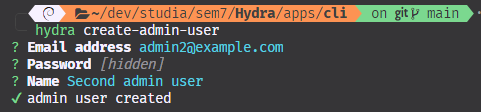
\includegraphics{cli/cli-questions.png}
  \caption{Example of \texttt{cli} application asking user for missing data}
\end{figure}

All of the values entered by the user are subjected to validation using the \texttt{class-validator} library \cite{class-validator}.

\begin{figure}[H]
  \centering
  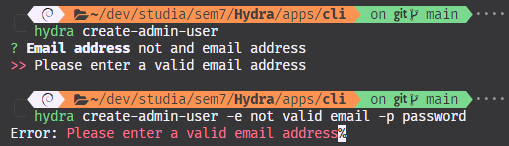
\includegraphics{cli/command-validation.png}
  \caption{Command input validation}
\end{figure}

Validation is checked when entering answer to a question and when the command is executed.
Checking the value when entering the answer to a question allows the user to correct the input before executing the command.
If validation fails when executing the command, the error message is displayed and the command will return with a non-zero exit code.


\end{document}